\section{Evaluation}

We ask: (RQ1) do practical projection boundaries admit target-achieving
collateral? (RQ2) do active witnesses recover missing passive coverage?
(RQ3) do separately specified semantic audits expose non-overlapping model gaps?
(RQ4) how safely and availably does one LLM edit configurations, including
against prior-workflow adaptations on the same Day-2 task? (RQ5) what are
the applicability and scaling limits?  The \emph{registered semantic model} is
the pre-specified, hash-frozen finite attribute universe, not a completeness
claim.  Full$_R$ evaluates its Envelope there; an out-of-contract Batfish audit
adds dimensions, and Full$_U$ is their fail-closed union.  Evidence is layered:
RQ1--RQ2 test compiler fidelity, RQ3 exposes independent model gaps, and RQ4
measures end-to-end release behavior with a sealed outcome oracle.  The frozen
and exploratory/developmental pools are never combined.

\subsection{Frozen public-corpus challenge and methods}

Before opening labels, we froze protocol \texttt{pathdelta-protocol-v1.0.0}, mechanism
hashes, source revisions, seeds, and analysis.  We freshly downloaded 64 Cisco
IOS scenarios from Cornetto~\cite{protogeros2026cornetto} and 32 Batfish policy
examples (4 Arista EOS, 28 Junos).  Sources and generated files are pinned and
hashed; no earlier PathDelta data or result is an input.

An Envelope-blind red-team prompt sees only intent and baseline and proposes
minimal, isolated, and adversarial edits.  We retain all outputs: nine calls
fail generation; 253 candidates apply, of which 178 achieve the target and 75
do not.  The registered model covers decision, local preference, communities,
and session; 58 goal candidates are safe and 120 have collateral.  Verdicts are
hashed before sealed labels are read.

RQ1 compares Goal-only, Write-scope, Visible+Scope, a \emph{VerifierLoop} that
checks target and differential behavior over operator-visible tests, a manually
completed \emph{OracleContract}, and Full$_R$, which
adds active witnesses, semantic frame, protected dependencies, and footprint.
The first three are diagnostic projections, not prior-system reproductions.
OracleContract is a non-deployable labeling upper bound written with the
evaluation model; Full$_R$ compiles from intent and pre-state before seeing a
candidate (median 131 obligations, P95 195).
Unsafe false acceptance (FA) is measured only among oracle target-achieving
unsafe candidates; safe false rejection (FR) is measured among oracle-safe
target-achieving candidates.  We use Wilson 95\% intervals and paired exact
McNemar tests with Holm correction.

Seed 83127 shuffles the 253 applicable candidates without labels and retains
128; labels opened later reveal 33 safe-goal, 56 unsafe-goal, and 39 non-goal
first candidates.  Six Agent128 arms replay the identical first patch; RAG
changes the prompt and is matched but not causal.  Iterative arms receive
patch-free counterexamples and may submit five baseline-relative patches.  All
use \texttt{deepseek-v4-flash}, temperature 0, and disabled thinking mode; we
separately record logical calls, backend attempts, retries, tokens, and latency.
Replay is deterministic on this frozen set, although candidate distribution
and repair availability remain endpoint- and prompt-specific.

\subsection{RQ1: semantic authority is not a projection}

Table~\ref{tab:external-main} gives the registered result.  Goal-only and
Write-scope accept all 120 collateral patches; visible verification accepts 12
(10\%).  Full$_R$ and OracleContract accept none and reject none of 58 safe
alternatives.  Full$_R$'s Wilson upper bounds are 3.10\% FA and 6.21\% FR; all
12 discordances with VerifierLoop favor Full$_R$ (exact $p=0.000488$,
Holm-adjusted $p=0.00293$).  The direction holds in both source groups.  Matching
the manual bound tests compilation within one model, not model completeness.
FA/FR denominators exclude the 75 non-goal candidates, which remain included
in the Agent128 analysis.

The 58 registered-safe alternatives span 51 scenarios, all three vendors, and all three
candidate modes (49 isolated, seven adversarial, and two minimal).  Zero FR
therefore does not mean comparison with one expected patch.

\begin{table}[t]
\caption{Registered public-corpus boundary study.}
\label{tab:external-main}
\centering
\footnotesize
\setlength{\tabcolsep}{3.1pt}
\begin{tabular}{lrrrr}
\toprule
Boundary & Unsafe acc. & FA & Safe rej. & FR \\
\midrule
Goal-only & 120/120 & 100\% & 0/58 & 0\% \\
Write-scope & 120/120 & 100\% & 0/58 & 0\% \\
Visible+Scope & 12/120 & 10\% & 0/58 & 0\% \\
VerifierLoop & 12/120 & 10\% & 0/58 & 0\% \\
OracleContract & 0/120 & 0\% & 0/58 & 0\% \\
\textbf{Full$_R$} & \textbf{0/120} & \textbf{0\%} & \textbf{0/58} & \textbf{0\%} \\
\bottomrule
\end{tabular}
\end{table}

The pre-specified 15-point superiority criterion was not met.  We therefore
restrict RQ1 to the observed closure of the 12 visible-test false accepts within
the registered model, rather than claim the pre-specified effect magnitude.
The paired difference remains statistically detectable; we did not tune the
registered mechanism or lower the gate.

Leave-one-out results further constrain the claim.  Removing the semantic
frame accepts all 120 registered-unsafe patches; removing active witnesses
accepts 12.  Removing dependency protection or footprint changes no verdict in
this public-corpus pool.  Those components may be prudent, but this experiment does
not establish their independent necessity.

\subsection{RQ2: coverage-directed witnesses}

Figure~\ref{fig:external-evidence} adds a missing-coverage study.  We delete
10\%, 25\%, or 50\% of passive records under random and adversarial removal,
with 20 replicates per condition.  Adversarial removal prioritizes sealed-oracle
collateral victims; it is a stress test, not a deployment distribution.
Passive-only FA rises from 12.7\% to 20.7\% under random removal and from
25.0\% to 82.5\% under adversarial removal.  Adding active witnesses holds mean
FA to 0.88--2.29\% and 4.17--5.0\%, respectively, with zero safe FR.  Active
Witnesses recover coverage but are not complete; classes absent from both models
remain outside the claim.

\begin{figure*}[t]
  \centering
  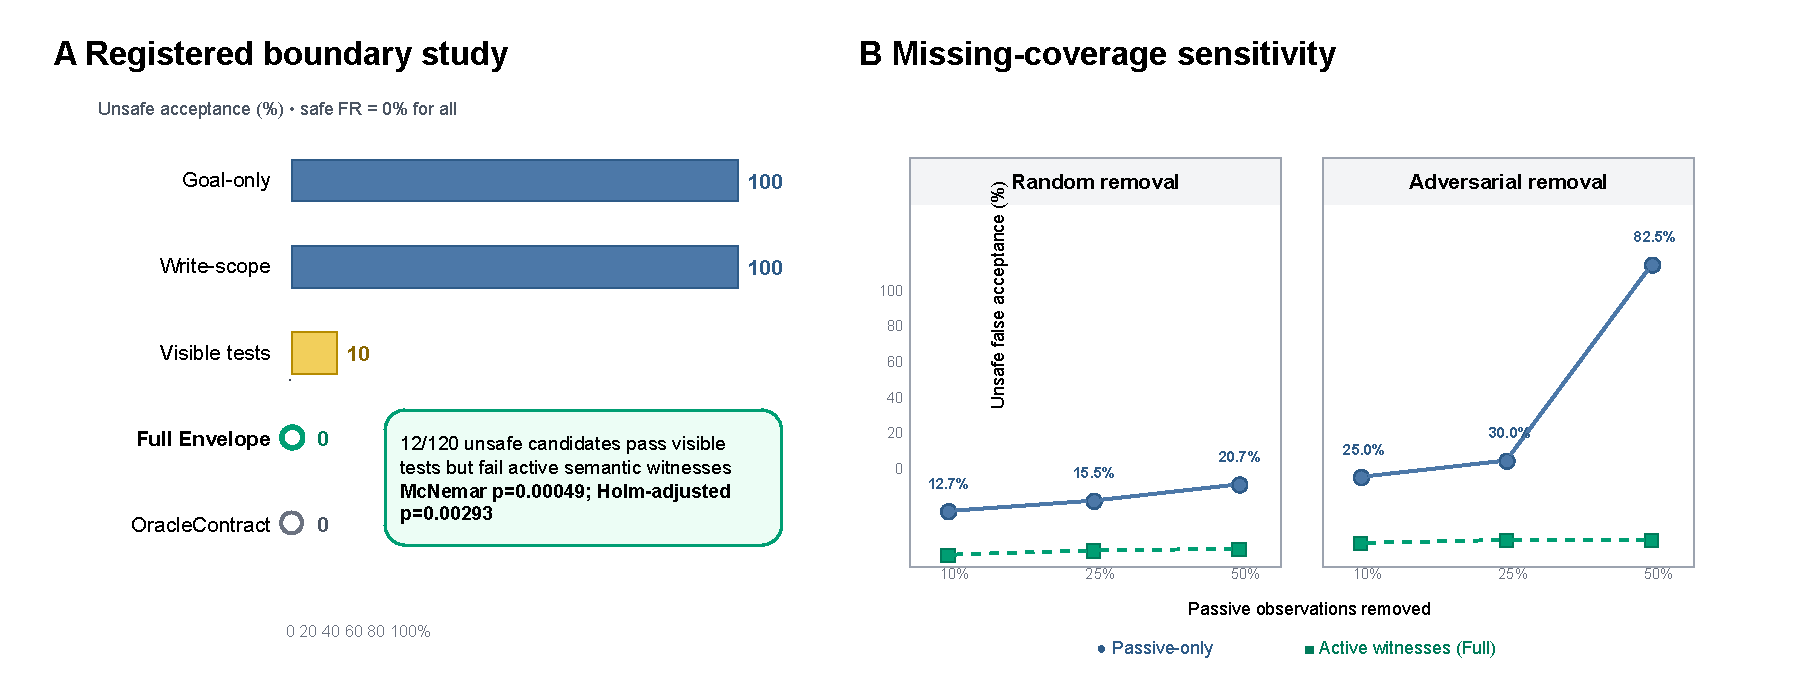
\includegraphics[width=0.98\textwidth]{figures/external_evidence.pdf}
  \caption{Registered public-corpus evidence.  (A) Full$_R$ closes 12 unsafe
  acceptances left by visible tests without rejecting registered-safe
  alternatives.  (B) active witnesses substantially reduce sensitivity to
  missing passive observations; all values are means over 20 replicates.
  Active witnesses are finite, not a completeness theorem, but remain at or
  below 5.0\% mean unsafe acceptance under every tested removal condition.}
  \label{fig:external-evidence}
\end{figure*}

\subsection{RQ3: separately specified models are complementary}

The registered oracle and Full$_R$ share a finite multi-vendor attribute
adapter.  To probe complementarity, we separately run Batfish queries outside
Full$_R$'s acceptance logic:
\texttt{searchRoutePolicies}/\texttt{compareRoutePolicies} over the frozen
candidates and additionally track metric and origin type.  Symbolic comparison
is applicable to 233/253 candidates and materializes 557 equivalence classes.
Twelve registered-safe candidates also change metric 200$\rightarrow$0 and
origin IGP$\rightarrow$EGP while changing authorized local preference;
Batfish conversely misses ten registered collateral cases.  Thus
Full$_R$=OracleContract establishes within-model consistency, not completeness.

One pair makes the gap concrete.  In Junos \texttt{09bea0}, a target term
changes local preference 200$\rightarrow$250 but also metric
200$\rightarrow$0 and origin IGP$\rightarrow$EGP, fields exposed only by the
Batfish audit.  In Arista \texttt{1dab61}, a shared action tags non-target
\texttt{10.100.0.0/16}; the registered frame rejects it, while the
target-scoped Batfish query does not classify it as unauthorized.  Neither
model subsumes the other.

Table~\ref{tab:cross-model} reports an exploratory audit on 162 jointly
applicable goal candidates, labeling a candidate unsafe if either model exposes
unauthorized behavior.  Full$_R$ and Batfish accept 12/119 and 10/119 unsafe,
respectively; their fail-closed conjunction (Full$_U$) accepts none and retains
all 43 cross-model-safe implementations.  Defined after the audit exposed the
gap, this union is not pooled with confirmation; it shows how explicit
obligations and provenance expose non-overlapping blind spots.

\begin{table}[t]
\caption{Exploratory cross-model audit on jointly applicable goal candidates.}
\label{tab:cross-model}
\centering
\footnotesize
\setlength{\tabcolsep}{3.6pt}
\begin{tabular}{lrrrr}
\toprule
Boundary & Unsafe acc. & FA & Safe rej. & FR \\
\midrule
Full$_R$ only & 12/119 & 10.1\% & 0/43 & 0\% \\
Batfish only & 10/119 & 8.4\% & 0/43 & 0\% \\
\textbf{Full$_U$ (AND)} & \textbf{0/119} & \textbf{0\%} & \textbf{0/43} & \textbf{0\%} \\
\bottomrule
\end{tabular}
\end{table}

\subsection{RQ4: end-to-end agent behavior}

\subsubsection{Agent128 safety and availability}

Table~\ref{tab:agent128} separates verified completion (VC),
goal-achieving collateral release (CR), failed-intent release (FI), terminal
transaction failure (TF), successful reject-to-safe repair, and attempt
exhaustion.  Direct and RAG release syntactic submissions, including non-goal
candidates.  Goal and write-scope release 61 and 59 collateral changes;
VerifierLoop reduces CR to five.  OracleContract and Full$_R$ release none in
the registered model; Full$_R$ repairs 16 first candidates and completes 49/128.

\begin{table}[t]
\caption{Agent128 end-to-end outcomes ($n=128$).}
\label{tab:agent128}
\centering
\scriptsize
\setlength{\tabcolsep}{2.5pt}
\begin{tabular}{lrrrrrr}
\toprule
Method & VC & CR & FI & TF & Repair & Exh. \\
\midrule
Direct replay & 33 & 56 & 39 & 0 & 0 & 0 \\
RAG one-shot & 16 & 48 & 63 & 1 & 0 & 0 \\
Goal-only & 43 & 61 & 0 & 0 & 10 & 24 \\
Write-scope & 39 & 59 & 0 & 0 & 6 & 30 \\
VerifierLoop & 40 & 5 & 0 & 0 & 7 & 83 \\
OracleContract & 45 & 0 & 0 & 0 & 12 & 83 \\
\textbf{Full$_R$} & \textbf{49} & \textbf{0} & \textbf{0} & \textbf{0} & \textbf{16} & \textbf{79} \\
\bottomrule
\end{tabular}
\end{table}

This is not ``safety for free.''  Full$_R$ fails closed in 79 events: 47 end
with semantic collateral and 32 still miss the target after five submissions.
Its higher VC than OracleContract is not attributed to the boundary because
revision calls are separate model samples after the paired first candidate.
The causal claim is confined to first-candidate acceptance; revision outcomes
measure operational behavior.

\textit{Post-freeze engineering analysis.}  Using the 79 exhaustions for
development, execution evidence and actionable transaction errors raise replay
to 128/128 without changing Full$_R$ acceptance.  Batfish then exposes 33
semantic failures and seven \na; frozen feedback repairs 32/33, so the
fail-closed union completes 120/128.  Agent128 uses 1,416 calls/6.40M tokens and
this replay adds 104 calls/1.04M tokens.  A label-independent 32-case holdout
completes 31/32 (one \na), with no measured unsafe release.  These results are
developmental, not confirmatory.

\subsubsection{Prior-workflow adaptations}

We adapt four workflows to the common task: the
classify--translate--generate--verify pipeline of
LLM-NetCFG~\cite{lira2024llmnetcfg}; INTA's fragment, retrieval, and refinement
stages~\cite{wei2025inta}; the verifier-guided prompt loop of CoSynth/Verified
Prompt Programming (CoSynth/VPP)~\cite{mondal2023router}; and the
inspect/edit/verify/rollback/submit agentic-repair loop
~\cite{asadli2026agentic} on Cornetto's public artifacts
~\cite{protogeros2026cornetto}.  They retain each paper's principal stages but
neither reproduce its native task nor rank the published systems.

We freshly select 48 public configurations, all file-disjoint and 46/48
topology-disjoint from controller development.  An excluded eight-case pilot
precedes the frozen 40-case split.  Arms share the model, temperature, baseline,
parsed context, transactions, 12-call/40k-token ceiling, and a sealed outcome
oracle consulted only after execution.  Only \system constructs active
witnesses; no arm sees a reference patch or oracle feedback.

Table~\ref{tab:external-methods} uses frozen Full$_R$; substituting Full$_U$,
defined only after RQ3 exposed a model gap, would make an exploratory repair
appear confirmatory.  Its results remain separate above.  VC is target-achieving
and oracle-safe, Unsafe is any released oracle-unsafe candidate, and Calls is
the per-case median.

\begin{table}[t]
\caption{Confirmatory common-task adaptations ($n=40$).}
\label{tab:external-methods}
\centering
\scriptsize
\setlength{\tabcolsep}{2.5pt}
\begin{tabular}{lrrrr}
\toprule
Method (adapted) & VC & Unsafe & Exh. & Calls \\
\midrule
LLM-NetCFG & 3 & 28 & 9 & 2.0 \\
INTA & 2 & 4 & 34 & 7.0 \\
CoSynth/VPP & 0 & 12 & 28 & 8.0 \\
Cornetto/Agentic & 18 & 10 & 12 & 9.0 \\
\textbf{\system Full$_R$} & \textbf{35} & \textbf{0} & \textbf{5} & \textbf{3.5} \\
\bottomrule
\end{tabular}
\end{table}

Against Cornetto/Agentic, \system reduces unsafe release by 25 points
(Holm $p=0.00391$; bootstrap 95\% CI 12.5--37.5) and raises VC by 42.5 points
($p=0.000221$; CI 25--60).  Unsafe reductions are Holm-significant against
LLM-NetCFG and CoSynth/VPP, but not INTA ($p=0.125$); the zero-unsafe Wilson
upper bound is 8.76\%.

\system completes 3/3 community, 4/4 legacy, 22/25 ordered-policy, and 6/8
shared-prefix cases with no measured unsafe release, using 171 calls versus
Cornetto/Agentic's 348.  These outcomes are specific to the common task and do
not rank the native systems.

In a paired trace, target \texttt{10.200.5.0/24} shares a list with three
non-target prefixes.  LLM-NetCFG and CoSynth/VPP release a shared-term edit
that changes all four preferences.  \system reports only the three observed
100$\rightarrow$150 deltas; the LLM's second attempt independently creates a
target-exclusive list and passes.  Feedback never names that list or command.

Of five \system exhaustions, three miss the target, one has a stale anchor, and
one retains shared-prefix collateral; all fail closed.  Pinned
Cornetto code and LLM-NetCFG artifacts guide their adaptations (no unlicensed
code copied); INTA and CoSynth/VPP are paper-faithful reimplementations because
no usable repository was available.  The manifest records provenance.

\subsection{RQ5: applicability and scale}

Batfish parses 234/253 candidates; 19 are \na, and a hard gate rejects three of
58 registered-safe candidates.  Symbolic comparison has 20/253 \na, never
promoted to PASS.  Single-process compiler time is 9.81~s at 100k FECs (100
objects), 25.83~s at 500 devices/100k FECs, and 90.92~s at the coupled
10k-object/100k-FEC point (42.63~MiB peak), excluding Batfish.  Agent128 LLM
latency P50/P95 is 2.07/3.55~s; Full$_R$ uses 343 calls and 1.54M tokens (12.0k
per case), excluding backend compute and price.  Rela/Kathara are not in these
scale counts.  The runner records backend attempts but does not aggregate
heterogeneous-container wall-clock, so LLM latency is not an end-to-end proxy.
